\documentclass[12pt, twoside]{article}
\input{../preamble}
\usepackage{pgfplots}
\pgfplotsset{compat=1.18}

\fancyhead[LE]{\thepage}
\fancyhead[RO]{Name: \hspace{4cm} \,\\ \hspace{2.9cm} \,}
\fancyhead[LO]{La Scuola d'Italia / Dr.\ Huson / IB Math \\* 1 April 2026}

\begin{document}
\subsubsection*{6.5 Classwork: Quadratic Functions and Symmetry}

\begin{enumerate}[itemsep=0.2cm]

%--- Problem 1: Graph to factored and standard form [7 marks] ---
\item The diagram shows the graph of a quadratic function with
$x$-intercepts at $(1, 0)$ and $(5, 0)$.

\begin{center}
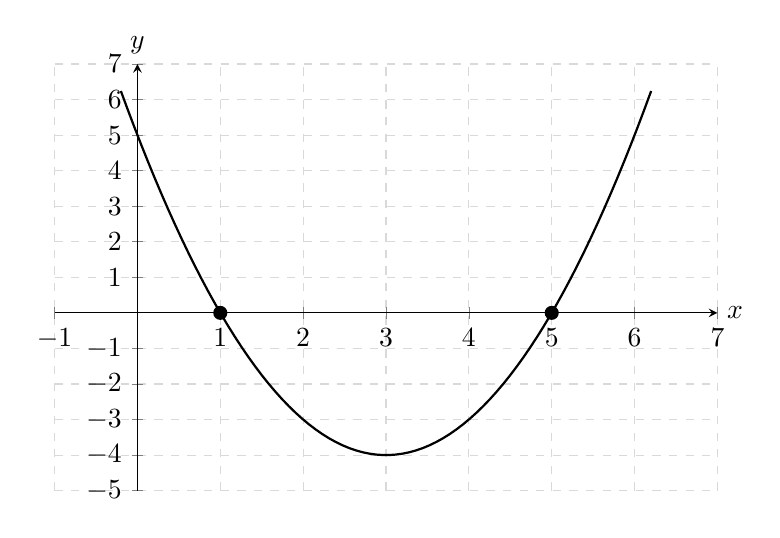
\begin{tikzpicture}
\begin{axis}[
  axis lines=middle,
  xlabel={$x$},
  ylabel={$y$},
  grid=both,
  grid style={dashed, gray!30},
  xmin=-1, xmax=7,
  ymin=-5, ymax=7,
  xtick={-1,0,...,7},
  ytick={-5,-4,...,7},
  width=10cm,
  height=7cm,
  every axis x label/.style={at={(ticklabel* cs:1.0)}, anchor=west},
  every axis y label/.style={at={(ticklabel* cs:1.0)}, anchor=south},
]
  % Parabola: y = x^2 - 6x + 5 = (x-1)(x-5), vertex (3,-4)
  \addplot[thick, domain=-0.2:6.2, samples=80] {x^2 - 6*x + 5};
  % x-intercepts
  \node[circle, fill, inner sep=1.8pt] at (axis cs:1,0) {};
  \node[circle, fill, inner sep=1.8pt] at (axis cs:5,0) {};
\end{axis}
\end{tikzpicture}
\end{center}

\begin{enumerate}[itemsep=0.15cm]
  \item Find the equation of the axis of symmetry. \hfill [1]
  \item Write the equation of the parabola in factored form, $y = (x - p)(x - q)$. \hfill [1]
  \item Expand to show that the equation is $y = x^2 - 6x + 5$. \hfill [2]
  \item Find the coordinates of the vertex. \hfill [2]
  \item Write down the $y$-intercept. \hfill [1]
\end{enumerate}

\begin{tikzpicture}
  \draw (0,0) rectangle (15.5,7);
  \foreach \y in {1,2,...,6} \draw [dotted] (0.5,\y)--(15,\y);
\end{tikzpicture}

\newpage

%--- Problem 2: Vertex form to standard form [7 marks] ---
\item The diagram shows the graph of $g(x) = -(x - 2)^2 + 9$.

\begin{center}
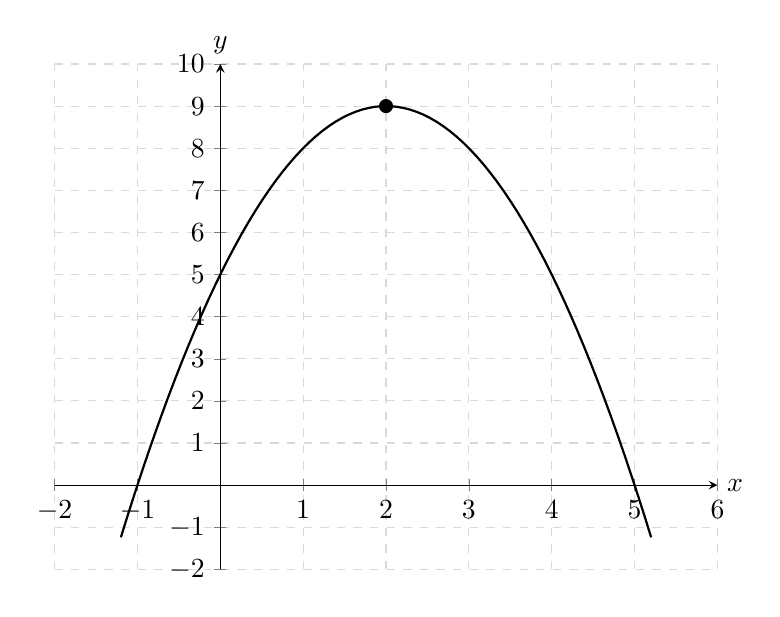
\begin{tikzpicture}
\begin{axis}[
  axis lines=middle,
  xlabel={$x$},
  ylabel={$y$},
  grid=both,
  grid style={dashed, gray!30},
  xmin=-2, xmax=6,
  ymin=-2, ymax=10,
  xtick={-2,-1,...,6},
  ytick={-2,-1,...,10},
  width=10cm,
  height=8cm,
  every axis x label/.style={at={(ticklabel* cs:1.0)}, anchor=west},
  every axis y label/.style={at={(ticklabel* cs:1.0)}, anchor=south},
]
  % Parabola: g(x) = -(x-2)^2 + 9, vertex (2,9), roots at x=-1 and x=5
  \addplot[thick, domain=-1.2:5.2, samples=80] {-(x-2)^2 + 9};
  % Vertex
  \node[circle, fill, inner sep=1.8pt] at (axis cs:2,9) {};
  % Label
  %\node[anchor=west] at (axis cs:0.5,1) {$g(x) = -(x - 2)^2 + 9$};
\end{axis}
\end{tikzpicture}
\end{center}

\begin{enumerate}[itemsep=0.15cm]
  \item Write down the coordinates of the vertex. \hfill [1]
  \item Write down the equation of the axis of symmetry. \hfill [1]
  \item Show that $g(x) = -x^2 + 4x + 5$. \hfill [2]
  \item Solve $g(x) = 0$ to find the $x$-intercepts. \hfill [3]
\end{enumerate}

\begin{tikzpicture}
  \draw (0,0) rectangle (15.5,9);
  \foreach \y in {1,2,...,8} \draw [dotted] (0.5,\y)--(15,\y);
\end{tikzpicture}

\newpage

%--- Problem 3: Standard form to factored and vertex form [7 marks] ---
\item The diagram shows part of the graph of $h(x) = x^2 - 2x - 3$.

\begin{center}
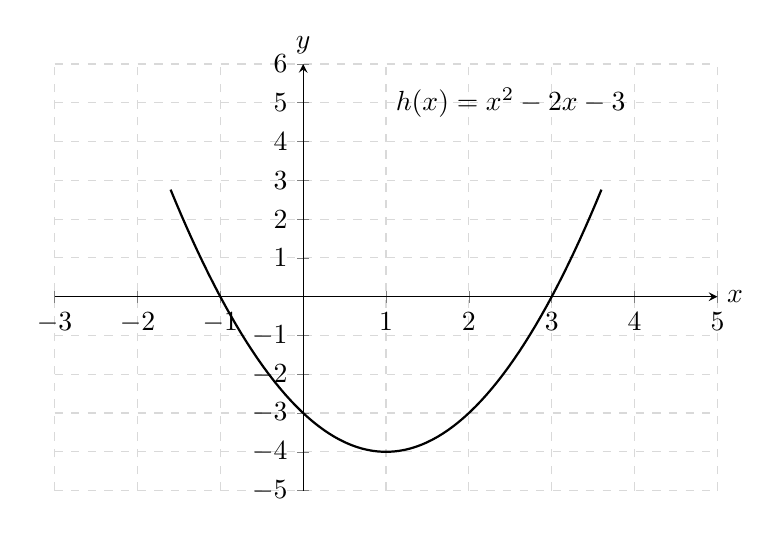
\begin{tikzpicture}
\begin{axis}[
  axis lines=middle,
  xlabel={$x$},
  ylabel={$y$},
  grid=both,
  grid style={dashed, gray!30},
  xmin=-3, xmax=5,
  ymin=-5, ymax=6,
  xtick={-3,-2,...,5},
  ytick={-5,-4,...,6},
  width=10cm,
  height=7cm,
  every axis x label/.style={at={(ticklabel* cs:1.0)}, anchor=west},
  every axis y label/.style={at={(ticklabel* cs:1.0)}, anchor=south},
]
  % Parabola: h(x) = x^2 - 2x - 3 = (x+1)(x-3), vertex (1,-4)
  \addplot[thick, domain=-1.6:3.6, samples=80] {x^2 - 2*x - 3};
  % Label
  \node[anchor=west] at (axis cs:1,5) {$h(x) = x^2 - 2x - 3$};
\end{axis}
\end{tikzpicture}
\end{center}

\begin{enumerate}[itemsep=0.15cm]
  \item Write $h(x)$ in factored form, $(x - p)(x - q)$. \hfill [2]
  \item Write down the $x$-intercepts of the parabola. \hfill [1]
  \item Find the equation of the axis of symmetry. \hfill [1]
  \item Find the coordinates of the vertex. \hfill [2]
  \item Write $h(x)$ in vertex form, $(x - h)^2 + k$. \hfill [1]
\end{enumerate}

\begin{tikzpicture}
  \draw (0,0) rectangle (15.5,7);
  \foreach \y in {1,2,...,6} \draw [dotted] (0.5,\y)--(15,\y);
\end{tikzpicture}

\newpage

%--- Problem 4: Sketch from factored form [7 marks] ---
\item Consider the quadratic function $p(x) = -x(x - 4)$ with domain $-1 \leq x \leq 5$.

\begin{enumerate}[itemsep=0.15cm]
  \item Write down the $x$-intercepts. \hfill [1]
  \item Find the equation of the axis of symmetry. \hfill [1]
  \item Find the coordinates of the vertex. \hfill [2]
  \item Expand to write $p(x)$ in the form $ax^2 + bx + c$. \hfill [1]
  \item On the grid below, sketch the graph of $p(x)$. Label the vertex
        and $x$-intercepts. \hfill [2]
        \item Write down the range of the function over the given domain. \hfill [1]
\end{enumerate}

\begin{center}
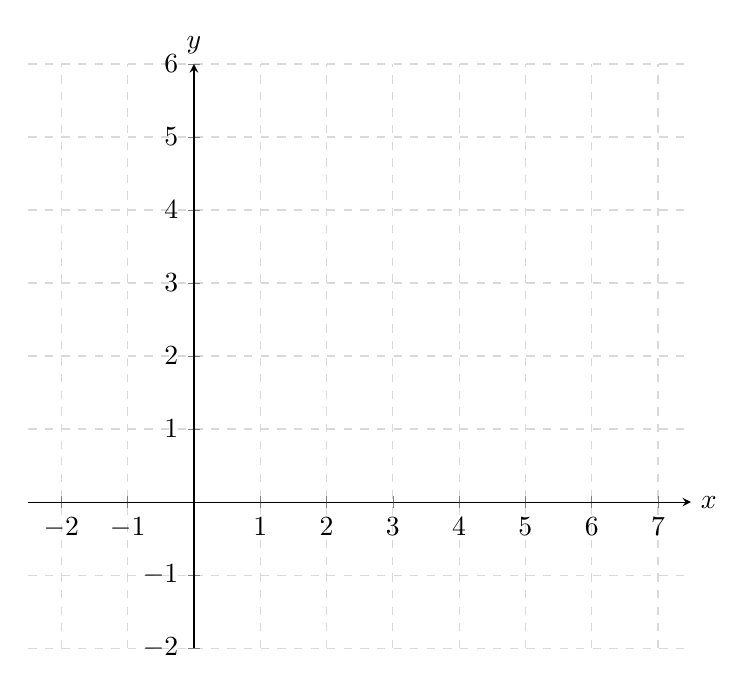
\begin{tikzpicture}
\begin{axis}[
  axis lines=middle,
  xlabel={$x$},
  ylabel={$y$},
  grid=both,
  grid style={dashed, gray!30},
  xmin=-2.5, xmax=7.5,
  ymin=-2, ymax=6,
  xtick={-2,-1,...,7},
  ytick={-2,-1,...,6},
  width=10cm,
  height=9cm,
  every axis x label/.style={at={(ticklabel* cs:1.0)}, anchor=west},
  every axis y label/.style={at={(ticklabel* cs:1.0)}, anchor=south},
]
  % Solution curve (commented out): p(x) = -x(x-4) = -x^2+4x, vertex (2,4)
  %\addplot[thick, domain=-0.5:4.5, samples=80] {-x^2 + 4*x};
\end{axis}
\end{tikzpicture}
\end{center}

\begin{tikzpicture}
  \draw (0,0) rectangle (15.5,7);
  \foreach \y in {1,2,3, 4, 5, 6} \draw [dotted] (0.5,\y)--(15,\y);
\end{tikzpicture}

\end{enumerate}
\end{document}

Solutions
  Problem 1 — Quadratic from graph, f(x) = x^2 - 6x + 5:
  - (a) Axis of symmetry: x = (1+5)/2 = 3
  - (b) Factored form: y = (x - 1)(x - 5)
  - (c) y = (x-1)(x-5) = x^2 - 5x - x + 5 = x^2 - 6x + 5
  - (d) Vertex: x = 3, y = 9 - 18 + 5 = -4. Vertex: (3, -4)
  - (e) y-intercept: x = 0, y = 5. Point: (0, 5)

  Problem 2 — Vertex form, g(x) = -(x-2)^2 + 9:
  - (a) Vertex: (2, 9)
  - (b) Axis of symmetry: x = 2
  - (c) g(x) = -(x^2 - 4x + 4) + 9 = -x^2 + 4x - 4 + 9 = -x^2 + 4x + 5
  - (d) -x^2 + 4x + 5 = 0 -> x^2 - 4x - 5 = 0 -> (x-5)(x+1) = 0
        x = 5 or x = -1. Intercepts: (-1, 0) and (5, 0)

  Problem 3 — Standard form, h(x) = x^2 - 2x - 3:
  - (a) h(x) = (x + 1)(x - 3) [i.e. p = -1, q = 3]
  - (b) x-intercepts: (-1, 0) and (3, 0)
  - (c) Axis of symmetry: x = (-1+3)/2 = 1
  - (d) h(1) = 1 - 2 - 3 = -4. Vertex: (1, -4)
  - (e) Vertex form: (x - 1)^2 - 4

  Problem 4 — Factored form, p(x) = -x(x - 4):
  - (a) x-intercepts: (0, 0) and (4, 0)
  - (b) Axis of symmetry: x = (0+4)/2 = 2
  - (c) p(2) = -2(2-4) = -2(-2) = 4. Vertex: (2, 4)
  - (d) p(x) = -x^2 + 4x
  - (e) Downward-opening parabola through (0,0) and (4,0) with vertex at (2,4)
